\documentclass[conference]{IEEEtran}
\IEEEoverridecommandlockouts
\usepackage{cite}
\usepackage{amsmath,amssymb,amsfonts}
\usepackage{algorithmic}
\usepackage{graphicx}
\usepackage{textcomp}
\usepackage{xcolor}
\usepackage{url}
\def\BibTeX{{\rm B\kern-.05em{\sc i\kern-.025em b}\kern-.08em
    T\kern-.1667em\lower.7ex\hbox{E}\kern-.125emX}}
\begin{document}

\title{Optimizing for Sequential Coherence and Playlist Coherence in Automatic Playlist Continuation}

\author{\IEEEauthorblockN{James Williams}
\IEEEauthorblockA{\textit{Whiting School of Engineering} \\
\textit{Johns Hopkins University}\\
Philadelphia, United States of America \\
jwill436@jh.edu}
}
\maketitle

\begin{abstract}
Automatic Playlist Continuation is naturally modeled as a sequence-to-sequence supervised learning task, and systems are 
commonly evaluated on metrics such as R-Precision and nDCG. These metrics account for the relevance of retrieved tracks, 
but they do not directly account for \textit{coherence}, or the degree to which a playlist forms a musically and sequentially 
consistent listening experience. This paper proposes modeling playlist coherence by assigning similarity scores to tracks based only
on co-occurrence statistics, and investigates the effect of including this metric in the training loss on nDCG and sequential coherence.
\end{abstract}

\begin{IEEEkeywords}
Automatic Playlist Continuation, Decoder-Only Transformers, Sequence-To-Sequence Modeling
\end{IEEEkeywords}

\section{Introduction}

Playlist continuation is a straightforward example of sequence-to-sequence modeling: Given some number of preceding songs, which songs should be played next?

Skilled disc jockeys are able to effectively adapt to variable crowd moods and responses through their choice and sequencing of tracks. 
Amateur disc jockeys merely curate playlists ahead of time, providing an experience no different than turning on the radio.
Radio stations and internet platforms profit by selling audience attention to advertisers or by charging subscription fees;
listeners devote their attention or dollars to these businesses as a consequence of playlist quality.

Automatic Playlist Continuation systems ingest data about playlists at the track level and recommend new tracks to append to the playlist. 
These systems are typically optimized for metrics like R-Precision and nDCG [3]. These metrics emphasize the correctness of 
predicted tracks based on the training data, but do not encode the ``coherence'' of the sequential listening experience provided by the new track, 
which can be ``vaguely defined as smooth transitions between tracks'' [2]. 

Large public datasets of real playlists are freely available for research purposes, such as the Million Playlist Dataset (MPD) [5],
consisting of 1,000,000 playlists from the Spotify music streaming service. The MPD includes complete per-track metadata for album, 
artist, and length, but does not include data such as genre, or any audio-derived features such as average loudness.

This paper can be reproduced via the following GitHub repository: \url{https://github.com/JamesCWilliams/Coherent_Automatic_Playlist_Continuation}.

\section{Related Work}

Schweiger et al. [1] observationally show that sequential variance in audio features and metadata between tracks in real 
playlists is meaningfully lower than variance in nonadjacent tracks, suggesting that sequentially-aware approaches should perform 
better than global approaches.

Schweiger et al. [2] provide stable definitions of playlist coherence based on audio features, and demonstrate that coherence 
increases with playlist length and so normalization is critical.

Bendada et al. [3] evaluate different algorithms for learning playlist representations solely from embeddings of songs 
and demonstrate that transformers achieve the largest precision, recall, R-precision, and nDCG among the methods evaluated.

Bendada et al. [4] describe a decoder-only architecture used in production for a real music streaming service.

Chen et al. [5] provide the Million Playlist Dataset (MPD), consisting of 1,000,000 playlists from the Spotify platform. 
These playlists were created between January 2010 and October 2017, and each playlist contains playlist metadata such as a 
title and an edit history, as well as individual track data, principally the track name and its position within the playlist.

\section{Research Project Problem}

This paper investigates the effect of incorporating a co-occurrence-based track similarity metric as a coherence term in 
the training loss on standard prediction accuracy metrics.

\section{Method}

A playlist is an ordered sequence of tracks $P = (t_1, t_2, \ldots, t_n)$ where each $t_i$ is drawn from the relevant universe 
of tracks $T$. The playlist continuation task is to learn a model that estimates the conditional probability 
$p(t_{i+1} \mid t_1, t_2, \ldots, t_i)$ for all valid $i$.

\subsection{Data}

This paper employs the MPD described in sections I and II. Only the track order information and unique track identifiers 
are retained for all analyses. While previous work such as [1] and [2] were able to employ the Spotify API to obtain more 
detailed per-track features, this author was unable to utilize the API.

Each playlist is converted into input-target pairs $(t_1, t_2, \ldots, t_{n-1}), (t_2, t_3, \ldots, t_n)$, with the model 
trained to predict the latter from the former. Special tokens for beginning-of-sequence, end-of-sequence, unknown track, 
and padding are injected into each sequence for ease of modeling. 

The dataset is split deterministically into training (80\%), validation (10\%), and testing (10\%) sets by the playlist identifier, where 
playlists shorter than a minimum threshold (2 tracks) are removed. Playlists are truncated to a maximum of 64 tokens (62 tracks),
and tracks which appear fewer than 3 times in the training set are replaced with the ``unknown'' token.

All data retrieval and preprocessing are performed in a streaming manner for efficiency.

\subsection{Model}

Following [4], this paper implements a decoder-only transformer language model. Each track token is mapped to a learned 
embedding vector, with positional embeddings added to preserve order. The resulting representation is then passed through a 
stack of transformer blocks that employ causal masking, ensuring that predictions depend only on previous tracks.

The final hidden states are projected to logits over $T$ via a learned linear layer.

Cross-entropy loss is used for model training.

\subsection{Coherence}

This paper introduces a track similarity metric based on playlist co-occurrence as a proxy for more detailed per-track features. 
Intuitively, tracks that co-occur more often should be more similar than tracks that co-occur less often. 
This metric requires only playlist data, unlike prior work that relied on audio features.

Track similarity is defined as:

\begin{equation}
\text{sim}(i, j) = \frac{\text{co-occurrence}(i, j)}{\sqrt{\text{occurrence}(i)\cdot\text{occurrence}(j)}}
\end{equation}

This cosine-style normalization assigns higher similarity to tracks that frequently co-occur. To improve training efficiency, a dense similarity 
matrix is precomputed before training.

Following the suggestion of [2], this paper focuses on the similarity of the final context track to the predicted next track as the training signal. 
Formally, for a prediction distribution $p(\cdot)$ over $T$ given some number of context tracks, the expected sequential 
coherence is $\mathbb{E}[C] = \sum_{t \in T} p(t)\,\text{sim}(t_\text{prev}, t)$. 
Maximizing this encourages coherent next-track predictions, so the coherence loss is defined as $\mathcal{L}_\text{coh} = -\mathbb{E}[C]$. 
The final training loss is

\begin{equation}
\mathcal{L} = \mathcal{L}_\text{CE} + \lambda\,\mathcal{L}_\text{coh},
\end{equation}

\noindent where $\lambda \geq 0$ is a regularization hyperparameter controlling the accuracy / coherence trade-off.

\section{Experiments}

\subsection{Setup}

Experiments use 8,000 randomly-selected playlists from the MPD as the training set, with tracks appearing fewer than three 
times removed from the vocabulary, yielding a vocabulary of 32,132 unique tracks. Sequences are truncated to a maximum length 
of 64 tokens, or 62 tracks plus the beginning-of-sequence and end-of-sequence tokens.

The model is a decoder-only transformer with $d_\text{model}=256$, 4 attention heads, 4 layers, and feed-forward dimension 512, 
trained for 20 epochs with the Adam optimizer at learning rate $3\times10^{-4}$, weight decay $10^{-2}$, and gradient clipping at norm 1.0; gradient
clipping is suggested by [3] and [4].

To characterize the accuracy / coherence trade-off, coherence weight $\lambda$ is swept across 13 values: 
$\{0, 0.05, 0.1, 0.2, 0.5, 1, 2, 5, 10, 15, 20, 25, 50\}$. Each $(\lambda, \text{seed})$ pair is trained independently 
across 10 random seeds, and results are reported as mean +/- standard deviation over those seeds. When $\lambda > 0$, 
the training objective adds the sequential coherence term. Evaluation coherence is always computed as the sequential 
metric (similarity between the preceding context track and the greedy-decoded prediction) regardless of $\lambda$, so results are directly comparable across the sweep.

\subsection{Results}

Table~\ref{tab:results} reports test-set metrics at the best validation checkpoint for each $\lambda$. 
Figure~\ref{fig:pareto} shows the Pareto frontier of nDCG@20 against eval coherence, with error bars showing standard deviations in 
nDCG@20 (y-axis) and coherence (x-axis) over the 10 seeds.

\begin{table}[ht]
\centering
\caption{Test-set metrics at the best validation checkpoint (mean over 10 seeds).}
\label{tab:results}
\begin{tabular}{r|cccc|c}
\hline
$\lambda$ & nDCG@1 & nDCG@5 & nDCG@10 & nDCG@20 & Coherence \\
\hline
0 & 0.284 & 0.294 & 0.295 & 0.296 & 0.001 \\
1 & 0.284 & 0.294 & 0.295 & 0.296 & 0.003 \\
2 & 0.284 & 0.294 & 0.295 & 0.296 & 0.007 \\
5 & 0.277 & 0.288 & 0.288 & 0.289 & 0.061 \\
10 & 0.274 & 0.286 & 0.286 & 0.287 & 0.080 \\
15 & 0.269 & 0.283 & 0.284 & 0.284 & 0.102 \\
20 & 0.250 & 0.276 & 0.276 & 0.277 & 0.234 \\
25 & 0.219 & 0.263 & 0.263 & 0.264 & 0.419 \\
50 & 0.178 & 0.253 & 0.254 & 0.255 & 0.693 \\
\hline
\end{tabular}
\end{table}

\begin{figure}[ht]
\centering
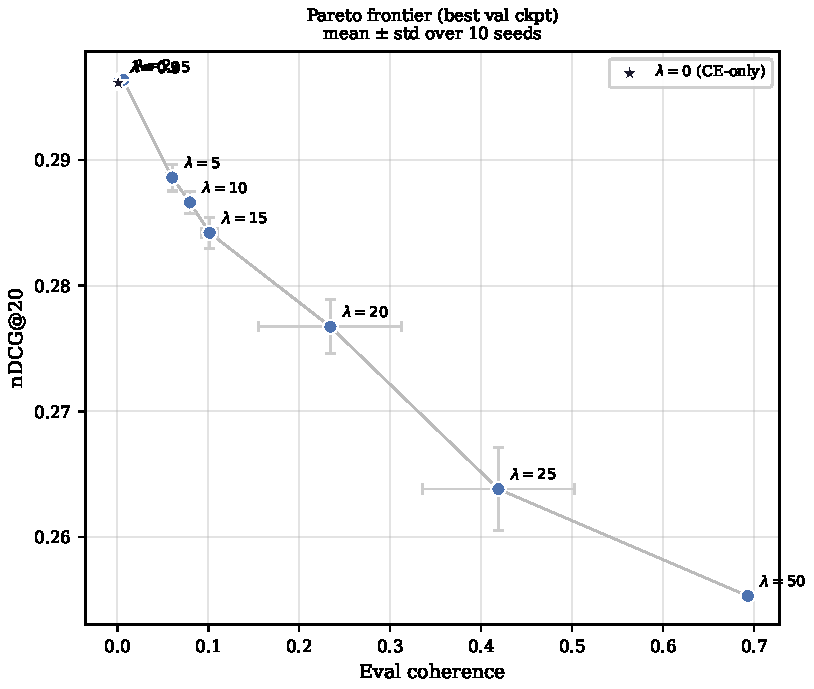
\includegraphics[width=\columnwidth]{../../saved_models/final_sweep/figures/pareto_frontier_best.pdf}
\caption{Pareto frontier of nDCG@20 vs.\ eval coherence across the $\lambda$ sweep (best validation checkpoint, 
mean +/- std over 10 seeds). Points are labeled by $\lambda$ value. The star marks the $\lambda=0$ cross-entropy baseline.}
\label{fig:pareto}
\end{figure}

\begin{figure}[ht]
\centering
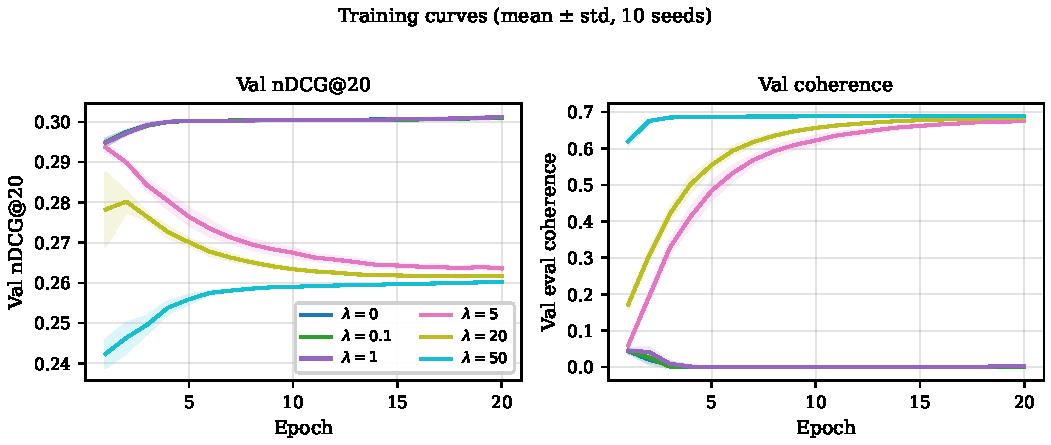
\includegraphics[width=\columnwidth]{../../saved_models/final_sweep/figures/training_curves.pdf}
\caption{Validation nDCG@20 (left) and eval coherence (right) across training epochs for a representative subset of $\lambda$ values. 
Shaded bands show +/- standard deviation across 10 seeds.}
\label{fig:training}
\end{figure}

\begin{figure}[ht]
\centering
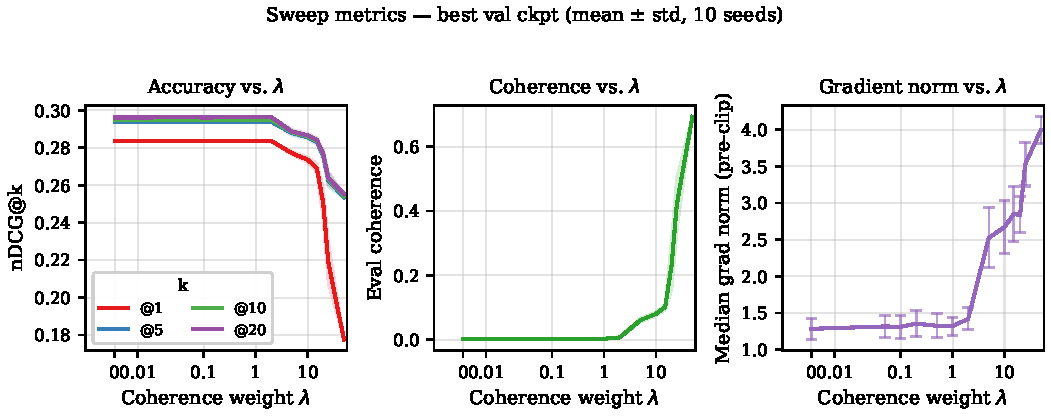
\includegraphics[width=\columnwidth]{../../saved_models/final_sweep/figures/metric_sweep_best.pdf}
\caption{nDCG@$k$ (left), eval coherence (center), and median pre-clip gradient norm (right) as a function of coherence 
weight $\lambda$, evaluated at the best validation checkpoint. Shaded bands and error bars show +/- 1 standard deviation across 10 seeds. 
The $\lambda$ axis uses a symmetric log scale with $\lambda=0$ at the origin.}
\label{fig:metrics}
\end{figure}

\subsection{Optimization Stability}

To assess whether the coherence gradient destabilizes training, the median per-epoch pre-clip gradient norm is recorded
for each seed run and aggregated across seeds. At $\lambda=0$ the median gradient norm is $1.28 +/- 0.15$. Norms remain near
this level for $\lambda\leq2$, then rise sharply at $\lambda=5$ ($2.53 +/- 0.41$) and continue
increasing to $3.99 +/- 0.18$ at $\lambda=50$. Gradient clipping at norm 1.0 limits the effect of these larger raw norms
on weight updates, and the low seed-to-seed variance in nDCG for all $\lambda$ values (Table~\ref{tab:results}) suggests
that training remains stable throughout the sweep.

\subsection{Prediction Diversity}

To measure whether the coherence regularizer reduces popularity bias, top-1 predictions are collected over all
valid token positions in the test set for a representative seed from each $\lambda$ value. Three statistics are reported:
The number of unique predicted tracks, the corresponding fraction of the 32,132-track vocabulary
(coverage), and normalized entropy $H_\text{norm} = H / \log|\mathcal{V}|$, where $H$ is the
Shannon entropy of the empirical prediction distribution. A fourth column reports the fraction of predictions
accounted for by the ten most frequently predicted tracks (top-10 concentration). Table~\ref{tab:diversity}
summarizes these statistics for five representative $\lambda$ values.

\begin{table}[ht]
\centering
\caption{Prediction diversity on the test set (greedy top-1, single representative seed per $\lambda$).}
\label{tab:diversity}
\begin{tabular}{r|r|r|r|r}
\hline
$\lambda$ & Unique & Coverage (\%) & $H_\text{norm}$ & Top-10 Conc.\ (\%) \\
\hline
0 & 39 & 0.12 & 0.011 & 99.9 \\
2 & 107 & 0.33 & 0.015 & 99.2 \\
5 & 902 & 2.81 & 0.066 & 93.7 \\
15 & 1,617 & 5.03 & 0.128 & 87.6 \\
50 & 11,064 & 34.43 & 0.659 & 31.1 \\
\hline
\end{tabular}
\end{table}

The baseline model ($\lambda=0$) exhibits popularity collapse: only 39 of 32,132 tracks are ever predicted,
and the ten most common predictions account for 99.9\% of all outputs. The dead zone ($\lambda \leq 2$)
provides no relief. In the moderate regime ($5 \leq \lambda \leq 15$), diversity improves substantially:
the number of unique predicted tracks grows by a factor of ${\approx}30$ relative to baseline and top-10 concentration
drops below 90\%, while nDCG@20 declines by only ${\approx}2$\%. At $\lambda=50$, 34\% of the vocabulary
is reached and entropy rises to 66\% of maximum, but at a cost of ${\approx}14$\% in nDCG@20.

\section{Discussion}

The results reveal three distinct operating regimes based on ranges of values for $\lambda$.

For $\lambda \leq 2$, the coherence loss provides no meaningful signal: eval coherence stays at ${\approx}0.005$,
indistinguishable from the baseline, while nDCG is unchanged. This suggests that at small weights the coherence gradient 
is too weak to compete with the cross-entropy term and the model effectively ignores it.

For $5 \leq \lambda \leq 15$, a moderate coherence improvement emerges: Eval coherence rises to ${\approx}0.10$ at a modest accuracy cost of ${\approx}2$\% in nDCG@20. 
Gradient norms roughly double relative to baseline but remain manageable under clipping. This regime represents the most favorable 
operating point if coherence is valued alongside accuracy.

For $\lambda \geq 20$, coherence rises substantially (${\approx}0.5$) but accuracy degrades sharply, 
with nDCG@20 falling ${\approx}10$\% below baseline. At $\lambda=50$ the standard deviation of coherence across seeds 
collapses to near zero (0.0001), indicating that the strong regularizer dominates the loss and drives all seeds to the 
same high-coherence but low-accuracy solution.

The three-regime structure is independently replicated in the diversity analysis. The coherence regularizer acts as
an implicit anti-popularity-bias term: In the moderate regime it reduces top-10 concentration from 99.9\% to below
90\% and increases unique predicted tracks by more than an order of magnitude relative to baseline, at the same
${\approx}2$\% nDCG cost already observed. This is a practically significant benefit beyond coherence alone, since
popularity-collapsed recommendations are less useful to users regardless of their coherence properties. The diversity
gain is therefore a second argument for the $5 \leq \lambda \leq 15$ operating point.

The co-occurrence similarity metric used here is a proxy for audio-based coherence, since the MPD does not provide
per-track audio features. The fact that optimizing this proxy produces measurable improvements in the eval metric 
suggests that playlist co-occurrence within the MPD encodes genuine musical affinity, consistent with the observational findings of 
[1]. However, the gap between co-occurrence similarity and true audio-feature coherence is unknown, and the absolute 
coherence values reached (up to 0.69 at $\lambda=50$) cannot be directly compared to the audio-based benchmarks in [2] 
without access to the Spotify API.

A limitation of this study is that the coherence evaluation metric is itself based on the same co-occurrence similarity 
used during training; only one matrix is precomputed for the entire dataset. A model trained with a high $\lambda$ 
may therefore score well on eval coherence by exploiting statistical regularities in the co-occurrence matrix rather than 
producing genuinely smoother playlists. Obtaining human judgments or audio-feature-based coherence scores for a 
subset of predictions would be necessary to validate whether the metric improvement reflects perceptible quality gains.

\section{Conclusion}

This paper demonstrates that co-occurrence-based sequential coherence can be incorporated as an auxiliary training 
signal for a decoder-only transformer playlist continuation model, and that doing so produces a clear Pareto frontier 
between ranking accuracy (nDCG) and eval coherence. The coherence regularizer is ineffective at small weights ($\lambda \leq 2$) 
and causes substantial degradation of nDCG at large weights ($\lambda \geq 20$). At intermediate weights ($5 \leq \lambda \leq 15$), 
coherence improves meaningfully while nDCG declines only modestly. An additional benefit in this regime is a
substantial reduction in popularity bias: the number of unique predicted tracks grows by more than an order of
magnitude relative to the collapsed baseline, suggesting that this range is a practical operating point for
applications where both sequential coherence and recommendation diversity matter.

Future work should investigate alternative coherence training signals. Prefix-mean similarity, which 
accounts for the full preceding context rather than only the immediately preceding track, could make the degradation of nDCG more modest.
Predicted playlists should be evaluated using audio-derived features or human judgments to establish whether co-occurrence coherence gains reflect 
perceptible listening quality improvements. Scaling to larger subsets of the MPD and larger model capacities would also 
be necessary to assess whether the accuracy / coherence trade-off holds at production scale.

\begin{thebibliography}{00}
\bibitem{b1} H. Schweiger, E. Parada-Cabaleiro, and M.
Schedl, “Does Track Sequence in User-generated Playlists Matter?”, in
Proc. of the 22nd Int. Society for Music Information Retrieval Conf.,
Online, 2021.
\bibitem{b2} H. Schweiger, E. Parada-Cabaleiro, and M. Schedl, ``The impact of playlist characteristics on coherence in user-curated music playlists,'' \textit{EPJ Data Sci.}, vol. 14, no. 24, 2025. https://doi.org/10.1140/epjds/s13688-025-00531-3
\bibitem{b3} Walid Bendada, Guillaume Salha-Galvan, Thomas Bouabça, and Tristan
Cazenave. 2023. A Scalable Framework for Automatic Playlist Continuation
on Music Streaming Services. In Proceedings of the 46th International ACM
SIGIR Conference on Research and Development in Information Retrieval
(SIGIR ’23), July 23–27, 2023, Taipei, Taiwan. ACM, New York, NY, USA,
11 pages. https://doi.org/10.1145/3539618.3591628
\bibitem{b4} Walid Bendada, Théo Bontempelli, Mathieu Morlon, Benjamin Chapus, Thibault Cador, Thomas Bouabça, and Guillaume Salha-Galvan.
2023. Track Mix Generation on Music Streaming Services using Transformers. In Seventeenth ACM Conference on Recommender Systems
(RecSys ‘23), September 18–22, 2023, Singapore. ACM, New York, NY, USA, 5 pages.
\bibitem{b5} C.W. Chen, P. Lamere, M. Schedl, and H. Zamani. Recsys Challenge 2018: Automatic Music Playlist Continuation. In Proceedings of the 12th ACM Conference on Recommender Systems (RecSys ’18), 2018.

\end{thebibliography}

\end{document}
